\documentclass[a4paper]{article}

\usepackage[margin=0.5cm]{geometry}
\usepackage{qtree}
\usepackage{color}
\usepackage{forest}
\usepackage{tikz}
\usepackage{listings}

\begin{document}
\begin{titlepage}
	\begin{center}
		\begin{figure}[t]
			\centering
			
\includegraphics[width=350px]{logo.PNG}
		\end{figure}
		
		\begin{center}
			\textsc{\Huge Programming Languages}
		\end{center}
		\begin{center}
			\textsc{\Huge COS 333}
		\end{center}
		\begin{center}		
			\textsc{\LARGE Practical Lab Experience 1:}		
		\end{center}
		\begin{center}		
			\textsc{\LARGE Research Assignment}		
		\end{center}
		
		\begin{flushright} \large
			Juan Jaques du Preez \newline \emph{u15189016} \newline
		\end{flushright}
\par\vspace{\fill}
{\large Date:}
\\
{\large \today}

	\end{center}
\end{titlepage}

\tableofcontents
\newpage

\section{Overview}
	\subsection{Overall UML Diagram}
		\begin{center}
			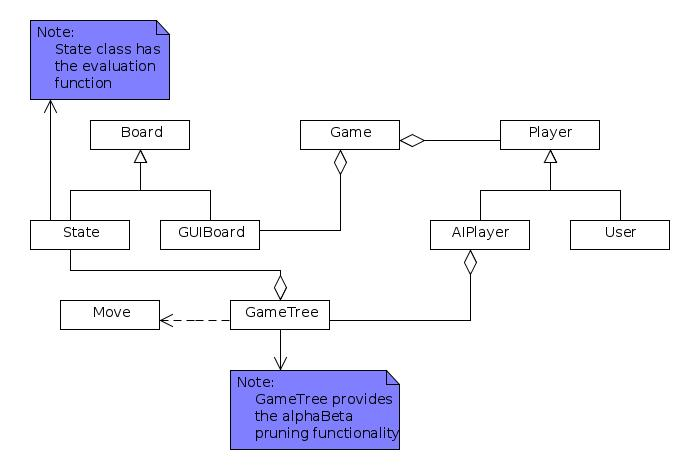
\includegraphics[width=350px]{fullUML.jpg}	
		\end{center}
	
	\subsection{Game Choice}
	I have decided to go with the \textsc{\LARGE Boa} game, because it seemed like more of a challenge.
	\subsection{Algorithm Choice}
	I chose to have \textsc{\LARGE alphaBeta pruning} functionality instead of just a simple minimax. The function itself and its 
	description is at the end of the document. The function can also be found in the GameTree.cpp file.
\section{Compile and Run Program}
For this project I used the Qt creator IDE, and the language of C++.
	\subsection{Compile}
	To compile the program, open a terminal and type in the following commands:
	\newline
	\newline
	\textbf{cd build-BaoGame-Desktop-Debug/} \newline
	\textbf{make} 
	\newline
	\newline
	Troubleshooting:\newline
	-If Qt creator is already installed on the system, it would be easier
		to open Qt creator and open the file /BaoGame/BaoGame.pro.
	-Otherwise, type 
	\newline
	\newline
	\textbf{whereis qmake}
	\newline
	\newline
	and copy/paste the path into the makefile at the following place:\newline
	\newline
	QMAKE = /usr/lib/qt/bin/qmake \newline
	\newline	
	which is where qmake is located on the lab computers.
	
	\subsection{Run}
	To run the program, make sure you are in the "build-BaoGame-Desktop-Debug/" directory
	and type: \newline
	\newline	
	\textbf{./BaoGame}
	\newline	
	\newline
	When the game is open, it is in User-vs-User mode. This means that the user defines all the moves that can be made. One can 		change the mode by going to the menu and creating a new game (User-vs-AI or AI-vs-AI), where you follow the instructions to 		specify ply depth of the AI or AIs.	
	\newline	
	\newline
	On the 	screen, you will see the possible moves displayed in yellow. A move is made by first clicking on one of the yellow-			highlighted holes and then selecting the direction by pressing the left or right buttons. Selecting right would mean that 			you choose to sow in the "right" direction. The actual sowing and capturing of seeds is displayed with the use of blue dots 		indicating which of the holes are in play.
	\newline	
	\newline
	The game also keeps track of how many seeds are in the stack of each player, as well as how many seeds are currently in the 			hand (the value on the right side of the board).
	\newline	
	\newline
	When an AI is playing, the alphaBeta pruning functionality can be followed in the terminal. It gives exactly which states it 	considers and which it prunes based on what knowledge.
	
	
	\subsection{Contact}
	If you cannot get the program to compile and run, please contact me: \newline
	Juan du Preez\newline
	078 141 0915\newline
	u15189016@tuks.co.za\newline
	juan.dupreez82@gmail.com
	
	\subsection{What does not work}
	To make your job easier, here is a list of things that do not work: \newline
	-There is no functionality for the Mtaji part of the game. I have attempted it, but failed. \newline
	-The "house" in Namua stage does not work. The game does not provide a option to stop if your last seed falls on the 				"house."\newline
	-The game, unfortunately, does not show which player is the current player.\newline
	-As soon as the seeds on each side runs out, the program stops.\newline
	-when compiling there will be a few warnings, but there should not be any errors. These warnings have to do with unused 			variables and virtual desturctors of abstract types.
	
	

\section{Evaluation Function}
	\subsection{The function}
	This function can be found in the BaoGame/State.cpp file:
	\begin{lstlisting}
int State::evaluate(bool player)
{
	//calculate if losing position 100 or -100
	if (isLosingPosition())
	{
		if (favouredPlayer == player)
			return 100;
        else return 0;
	}
	
	//weights
    const float countSeedWeight = 30.0;
    const float frontRowWeight = 20.0;
    const float backRowWeight= 10.0;
    const float frontRowOccWeight = 15.0;
    const float backRowOccWeight= 5.0;
    const float captureWeight = 20.0;
	
	
	//count seeds for each player
    float countSeed;
	int p1 = 0;
	for (int i = 0; i < 8; i++)
	{
		p1 += board[2][i] + board[3][i];
	}
	int p2 = 0;
	for (int i = 0; i < 8; i++)
	{
		p2 += board[0][i] + board[1][i];
	}
    if (player == PLAYER1) countSeed = 1.0 * (p1 / (p1 + p2));
    else countSeed = 1.0 * (p2 / (p1 + p2));
	
	//count seeds in front rows and back rows respectively
    float frontRow;
    float backRow;
	p1 =0;
	int p1b = 0;
	for (int i = 0; i < 8; i++)
	{
		p1 += board[2][i];
		p1b += board[3][i];		
	}
	p2 = 0;
	int p2b = 0;
	for (int i = 0; i < 8; i++)
	{
		p2 += board[1][i];
		p2b += board[0][i];
	}
	if (player == PLAYER1) 
	{
        frontRow = 1.0 * (p1 / (p1 + p2));
        if (p1b + p2b != 0) backRow = 1.0 * (p1b / (p1b + p2b));
        else backRow = 0.5;
	}
	else 
	{
        frontRow = 1.0 * (p2 / (p1 + p2));
        if (p1b + p2b != 0) backRow = 1.0 * (p2b / (p1b + p2b));
        else backRow = 0.5;
	}		
	
	//count how many holes are occupied in back row and front rows
    float frontRowOcc;
    float backRowOcc;
	p1 =0;
	p1b = 0;
	for (int i = 0; i < 8; i++)
	{
		if (board[2][i] != 0) p1++;
		if (board[3][i] != 0) p1b++;
	}
	p2 = 0;
	p2b = 0;
	for (int i = 0; i < 8; i++)
	{
		if (board[1][i] != 0) p2++;
		if (board[0][i] != 0) p2b++;
	}	
	if (player == PLAYER1) 
	{
        frontRowOcc = 1.0 * (p1 / 8);
        backRowOcc =1.0 * (p1b / 8);
	}
	else 
	{
        frontRowOcc = 1.0 * (p2 / 8);
        backRowOcc = 1.0 * (p2b / 8);
	}	
	
	//count the number of seeds each player can capture
    float capture = 0.5;
    if (!isTakasa())
    {
        p1 =0;
        p2 = 0;
        for (int i = 0; i < 8; i++)
        {
            if (board[2][i] != 0 && board[1][i] != 0)
            {
                p1 += board[1][i];
                p2 += board[2][i];
            }
        }
        if (player == PLAYER1) capture = 1.0 * (p1 / (p1 + p2));
        else capture = 1.0 * (p2 / (p1 + p2));
    }
	
	//return weighted sum
	return countSeedWeight * countSeed
		+ frontRowWeight * frontRow
		+ backRowWeight * backRow		
		+ frontRowOccWeight * frontRowOcc
		+ backRowOccWeight * backRowOcc
		+captureWeight * capture;
}
	\end{lstlisting}

	\subsection{Description of Evaluation function}
	In this function, there are six different aspects of a particular board state that I considered. Each of these six 
	apects are then multiplied with a pre-determined weight which I have assigned to them based on how important I think the 			step is.  Notice that the total at the end can be any number between 0 and 100. The function first checks if the state is in 	a losing position. If the current player is the loser,then the evaluation is 0. If the other player has lost the game, then 		the evaluation is set to 100. In order to demonstrate this, the following board state will be used:
	\newline
	\newline
	0 0 0 0 0 0 0 0\newline
	0 2 2 6 0 0 0 0\newline
	1 1 1 1 0 2 2 0\newline
	1 1 1 0 0 0 0 0\newline
	with regards to player1	(the player at the bottom)
	\newline
	\newline
	The six aspects are described as follows:
	\subsubsection{the number of seeds on each side of the board}
	The total number of seeds is counted for each side. Then player1's total is divided by the total of both. So\newline				11/(10+11) = 11/21 = 0.524 \newline This is then multiplied with the constant weight of 30 to get 15.714.
	\subsubsection{the number of seeds in each front row}
	The same is then done for the first row or top row of each player. This is done because the front row seeds are more 
	valuable than those in the back row.\newline
	8/(8+10) = 8/18 = 0.444\newline
	weighted: 20*0.444 = 8.889
	\subsubsection{the number of seeds in each back row}
	These back row seeds still have some value and also need to be calculated.\newline
	3/3 = 1\newline
	weighted: 10*1 = 10
	\subsubsection{the distribution of seeds in each front row}
	This part of the function counts how many non-empty holes there are in the front row and gives it in a ratio of x/8. This
	is done to see how distributed the seeds are. It is not helpful when you have 20 seeds, but they are all accumulated in
	a single hole. \newline
	6/8 = 0.75 \newline
	weighted: 15*0.75 = 11.25
	\subsubsection{the distribution of seeds in each back row}
	This is then done for the bottom hole as well.\newline
	3/8 = 0.375\newline
	weighted: 5*0.375 = 1.875
	\subsubsection{possible captures}
	The total number of seeds that can a player can capture is summed up for each player. Then the total for player1 is divided 		by the total again.  \newline
	player1 can capture: 2+2+6 = 10\newline
	player2 can capture: 1+1+1 = 3\newline
	10/(10+3) = 10/13 = 0.769\newline
	weighted: 20*0.769 = 15.385
	\subsection{Finally}
	At the end, all the weighted values are added together and truncated to form an integer value which is the final evaluated 			value:\newline
	15.714+8.889+10+11.25+1.875+15.385 = 63.113 = 63
	\subsection{Please Note:}
	I have not researched methods of calculating the state of a Bao game. I wanted to play the game myself and see what I come 			up with before I follow someone else's line of thought. Thus, my evaluation function may be trivial or incomplete, but it is	 	my own work.
	

\section{AlphaBeta pruning function}
This function can be found in BaoGame/gametree.cpp:\newline
\begin{lstlisting}
int GameTree::alphaBetaPruning(State* cur, int curDepth)
{
//used for displaying tree
	for (int i = 0; i < curDepth; i++)
	cout << "\t\t";
	cout << "depth " << curDepth << ": ";
	cur->print();

	if (curDepth == maxDepth)
    {
		cur->evaluation = cur->evaluate(player);
		return cur->evaluate(player);
    }
	
	if (cur->isMaxNode) cur->evaluation = -101;
    else cur->evaluation = 101;
	
	//generate list of moves
	vector<Move* >* moves = getPossibleMoves(cur);
	int tmp;
    bool prune;
	
	//for every move
	for (int i = 0; i < moves->size(); i++)
	{
		//add to children = get Next State(curstate, move[i])
		cur->children.push_back(getNextState(cur, (*moves)[i]));
		
		//add current alphaBeta value to stack
		if (cur->isMaxNode) 
		{
            alphaValues.push_back(cur->evaluation);
		}
		else 
		{
            betaValues.push_back(cur->evaluation);
		}

        //recursive call
        tmp = alphaBetaPruning(cur->children[i], curDepth + 1);
		
		//cur.alphaBeta value = max or min (tmp, cur.alphaBetaValue)
		if (cur->isMaxNode)
		{
			//find maximum of two values
			if (tmp > cur->evaluation) cur->evaluation = tmp;		
			//compare tmp to previous Beta values
			prune = compareBeta(tmp);
		}
		else
		{
			//find minimum of two values
			if (tmp < cur->evaluation) cur->evaluation = tmp;
			//compare tmp to previous alpha values
			prune = compareAlpha(tmp);
		}	
		
		//remove current alphaBeta value from stack
		if (cur->isMaxNode) 
		{
            alphaValues.pop_back();
		}
		else 
		{
            betaValues.pop_back();
		}
		
		//if (prune) delete moves and return temp
		if (prune)
		{
			for (int i = 0; i < moves->size(); i++)
				delete (*moves)[i];
			delete moves;
            //give status of pruning
            cout << "in abpruning: decided to prune because of " << tmp << endl;
			return tmp;
		}
	}
	//delete moves
	for (int i = 0; i < moves->size(); i++)
		delete (*moves)[i];
	delete moves;

	return cur->evaluation;
}

bool GameTree::compareAlpha(int x)
{
	//	"Search is discontinued below any Min node
	//	having a Beta value less than or equal to the Alpha
	//	value of any of its Max node ancestors"
	for (int i = 0; i < alphaValues.size(); i++)
		if (x <= alphaValues[i]) return true;
	return false;
}

bool GameTree::compareBeta(int x)
{
	// 	Search is discontinued below any Max node
	// 	having an Alpha value greater than or equal to
	//	the Beta value of any of its Min node ancestors
	for (int i = 0; i < betaValues.size(); i++)
		if (x >= betaValues[i]) return true;
	return false;	
}
\end{lstlisting}


\section{Rules of Bao}
\subsection{Namua Stage}
(as stated in spec:)\newline
• you have to capture if you can\newline
• entering captured seeds must be done in the front row from the first hole from the left or right\newline
• you have no choice whether to start from the left or right when:\newline
• you captured a kichwa or kimbi hole\newline
• you have already sown in a direction\newline
• if the last seed ends in an occupied hole, capture the opposing seeds\newline
• if there is nothing in the opposing hole, take the seeds from you holeand sow them in the same direction\newline
• your move ends when your last seed falls in an empty hole.\newline
\subsection{Mtaji Stage}
(as stated in spec:)\newline
• sow seeds from a hole (that may be a hole from the front or back row)\newline
• the last seed from that hole must end in a hole in the front row having one or more seeds\newline
• there must be one or more seeds in the opposing hole (mtaji)\newline
• the seeds in the mtaji are captured\newline
• playing singletons (holes with only one seed in it) is not allowed\newline
• if there is no mtaji, you play takasa (which will be explained later)\newline
\end{document}
